% answers.tex —— 2007 年·全国大纲卷Ⅱ·理科 · 参考答案与详细解析片段
% 由 tools/generate_projects.py 依来源总账自 2007/2007_数学真题_全国2理_试题.md + 2007/2007_数学真题_全国2理_解析正文.md + 2007/2007_数学真题_全国2理_答案要点.md 生成，勿手改（改源 MD 后重跑）


\begin{gktip}
固定源 PDF 为印刷页码 363–364 的两页题面，不附答案。以下解析均依据固定源独立复算；第 19 题图形在 LaTeX 工程中以 TikZ/PGFPlots 矢量源重绘。
\end{gktip}

\begin{answer}
\gksolhead{1}{}

\textbf{题目}：

$\sin210^\circ=$\mbox{（　　）}

（A）$\dfrac{\sqrt3}{2}$\quad（B）$-\dfrac{\sqrt3}{2}$\quad（C）$\dfrac12$\quad（D）$-\dfrac12$

\Needspace{4\baselineskip}
\textbf{解析}

\nopagebreak[4]
\[
\sin210^\circ=-\sin30^\circ=-\frac12
\]
。

\gkanswer{答案：B}

\end{answer}
\begin{answer}
\gksolhead{2}{}

\textbf{题目}：

函数 $f(x)=|\sin x|$ 的一个单调递增区间是\mbox{（　　）}

（A）$\left(-\dfrac\pi4,\dfrac\pi4\right)$\quad（B）$\left(\dfrac\pi4,\dfrac{3\pi}4\right)$\quad（C）$\left(\pi,\dfrac{3\pi}2\right)$\quad（D）$\left(\dfrac{3\pi}2,2\pi\right)$

\Needspace{4\baselineskip}
\textbf{解析}

与全国卷Ⅱ文科第 3 题相同，$|\sin x|$ 在 $(\pi,3\pi/2)$ 上递增。

\gkanswer{答案：C}

\end{answer}
\begin{answer}
\gksolhead{3}{}

\textbf{题目}：

设复数 $z$ 满足 $\dfrac{1+2i}{z}=i$，则 $z=$\mbox{（　　）}

（A）$-2+i$\quad（B）$-2-i$\quad（C）$2-i$\quad（D）$2+i$

\Needspace{4\baselineskip}
\textbf{解析}

\nopagebreak[4]
\[
\frac{1+2i}{z}=i\Longrightarrow z=\frac{1+2i}{i}=2-i
\]
。

\gkanswer{答案：C}

\end{answer}
\begin{answer}
\gksolhead{4}{}

\textbf{题目}：

以下四个数中的最大者是\mbox{（　　）}

（A）$(\ln2)^2$\quad（B）$\ln(\ln2)$\quad（C）$\ln\sqrt2$\quad（D）$\ln2$

\Needspace{4\baselineskip}
\textbf{解析}

与全国卷Ⅱ文科第 4 题相同，最大者为 $\ln2$。

\gkanswer{答案：D}

\end{answer}
\begin{answer}
\gksolhead{5}{}

\textbf{题目}：

在 $\triangle ABC$ 中，已知 $D$ 是 $AB$ 边上一点，若 $\overrightarrow{AD}=2\overrightarrow{DB}$，$\overrightarrow{CD}=\dfrac13\overrightarrow{CA}+\lambda\overrightarrow{CB}$，则 $\lambda=$\mbox{（　　）}

（A）$\dfrac23$\quad（B）$\dfrac13$\quad（C）$-\dfrac13$\quad（D）$-\dfrac23$

\Needspace{4\baselineskip}
\textbf{解析}

\Needspace{5\baselineskip}
由 $D=(A+2B)/3$ 得

\nopagebreak[4]
\[
\overrightarrow{CD}=\frac13\overrightarrow{CA}+\frac23\overrightarrow{CB}
\]
，

故 $\lambda=2/3$。

\gkanswer{答案：A}

\end{answer}
\begin{answer}
\gksolhead{6}{}

\textbf{题目}：

不等式 $\dfrac{x-1}{x^2-4}>0$ 的解集为\mbox{（　　）}

（A）$(-2,1)$\quad（B）$(2,+\infty)$\quad（C）$(-2,1)\cup(2,+\infty)$\quad（D）$(-\infty,-2)\cup(1,+\infty)$

\Needspace{4\baselineskip}
\textbf{解析}

作符号表，$\dfrac{x-1}{x^2-4}>0$ 的解集为 $(-2,1)\cup(2,+\infty)$。

\gkanswer{答案：C}

\end{answer}
\begin{answer}
\gksolhead{7}{}

\textbf{题目}：

已知正三棱柱 $ABC-A_1B_1C_1$ 的侧棱长与底面边长相等，则 $AB_1$ 与侧面 $ACC_1A_1$ 所成角的正弦等于\mbox{（　　）}

（A）$\dfrac{\sqrt6}{4}$\quad（B）$\dfrac{\sqrt{10}}4$\quad（C）$\dfrac{\sqrt2}2$\quad（D）$\dfrac{\sqrt3}2$

\Needspace{4\baselineskip}
\textbf{解析}

\Needspace{5\baselineskip}
取底面边长和侧棱均为 $1$。$AB_1$ 的方向向量与侧面 $ACC_1A_1$ 的法向量作线面角计算，得到正弦为

\nopagebreak[4]
\[
\frac{\sqrt3}{2\sqrt2}=\frac{\sqrt6}{4}
\]
。

\gkanswer{答案：A}

\end{answer}
\begin{answer}
\gksolhead{8}{}

\textbf{题目}：

已知曲线 $y=\dfrac{x^2}{4}-3\ln x$ 的一条切线的斜率为 $\dfrac12$，则切点的横坐标为\mbox{（　　）}

（A）$3$\quad（B）$2$\quad（C）$1$\quad（D）$\dfrac12$

\Needspace{4\baselineskip}
\textbf{解析}

\nopagebreak[4]
\[
y'=\frac{x}{2}-\frac3x
\]
。

令 $y'=1/2$，得 $x^2-x-6=0$，取正根 $x=3$。

\gkanswer{答案：A}

\end{answer}
\begin{answer}
\gksolhead{9}{}

\textbf{题目}：

把函数 $y=e^x$ 的图象按向量 $\boldsymbol a=(2,3)$ 平移，得到 $y=f(x)$ 的图象，则 $f(x)=$\mbox{（　　）}

（A）$e^{x-3}+2$\quad（B）$e^{x+3}-2$\quad（C）$e^{x-2}+3$\quad（D）$e^{x+2}-3$

\Needspace{4\baselineskip}
\textbf{解析}

\Needspace{5\baselineskip}
向量 $(2,3)$ 平移后，$x$ 坐标减 $2$、$y$ 坐标加 $3$，所以

\nopagebreak[4]
\[
f(x)=e^{x-2}+3
\]
。

\gkanswer{答案：C}

\end{answer}
\begin{answer}
\gksolhead{10}{}

\textbf{题目}：

从 $5$ 位同学中选派 $4$ 位同学在星期五、星期六、星期日参加公益活动，每人一天，要求星期五有 $2$ 人参加，星期六、星期日各有 $1$ 人参加，则不同的选派方法共有\mbox{（　　）}

（A）$40$ 种\quad（B）$60$ 种\quad（C）$100$ 种\quad（D）$120$ 种

\Needspace{4\baselineskip}
\textbf{解析}

\Needspace{5\baselineskip}
选星期五的两人有 $\binom52$ 种，再从剩余三人中有序选星期六、星期日两人，方法数为

\nopagebreak[4]
\[
\binom52\cdot3\cdot2=60
\]
。

\gkanswer{答案：B}

\end{answer}
\begin{answer}
\gksolhead{11}{}

\textbf{题目}：

设 $F_1,F_2$ 分别是双曲线 $\dfrac{x^2}{a^2}-\dfrac{y^2}{b^2}=1$ 的左、右焦点。若双曲线上存在点 $A$，使 $\angle F_1AF_2=90^\circ$，且 $|AF_1|=3|AF_2|$，则双曲线离心率为\mbox{（　　）}

（A）$\dfrac{\sqrt5}{2}$\quad（B）$\dfrac{\sqrt{10}}2$\quad（C）$\dfrac{\sqrt{15}}2$\quad（D）$\sqrt5$

\Needspace{4\baselineskip}
\textbf{解析}

\Needspace{5\baselineskip}
设 $u=|AF_2|$，则 $|AF_1|=3u$。因 $\angle F_1AF_2=90^\circ$ 且 $F_1F_2=2c$，

\nopagebreak[4]
\[
10u^2=4c^2,\qquad 2u=2a
\]
，

故 $e=c/a=\sqrt{10}/2$。

\gkanswer{答案：B}

\end{answer}
\begin{answer}
\gksolhead{12}{}

\textbf{题目}：

设 $F$ 为抛物线 $y^2=4x$ 的焦点，$A,B,C$ 为该抛物线上三点。若 $\overrightarrow{FA}+\overrightarrow{FB}+\overrightarrow{FC}=0$，则 $|\overrightarrow{FA}|+|\overrightarrow{FB}|+|\overrightarrow{FC}|=$\mbox{（　　）}

（A）$9$\quad（B）$6$\quad（C）$4$\quad（D）$3$

\Needspace{4\baselineskip}
\textbf{解析}

设抛物线参数为 $P(t)=(t^2,2t)$，则 $\overrightarrow{FP}=(t^2-1,2t)$，其长度为 $t^2+1$。向量和为零给出参数和为零、平方和为 $3$，所以长度和为 $6$。

\gkanswer{答案：B}

\end{answer}
\begin{answer}
\gksolhead{13}{}

\textbf{题目}：

$(1+2x^2)\left(x-\dfrac1x\right)^8$ 的展开式中常数项为\gkblank{}。（用数字作答）

\Needspace{4\baselineskip}
\textbf{解析}

\Needspace{5\baselineskip}
常数项为

\nopagebreak[4]
\[
\binom84+2\binom85(-1)=70-112=-42
\]
。

\gkanswer{答案：$-42$}

\end{answer}
\begin{answer}
\gksolhead{14}{}

\textbf{题目}：

在某项测量中，测量结果 $\xi$ 服从正态分布 $N(1,\sigma^2)\ (\sigma>0)$。若 $\xi$ 在 $(0,1)$ 内取值的概率为 $0.4$，则 $\xi$ 在 $(0,2)$ 内取值的概率为\gkblank{}。

\Needspace{4\baselineskip}
\textbf{解析}

正态分布关于均值 $1$ 对称，$P(1<\xi<2)=P(0<\xi<1)=0.4$，故 $P(0<\xi<2)=0.8$。

\gkanswer{答案：$0.8$}

\end{answer}
\begin{answer}
\gksolhead{15}{}

\textbf{题目}：

一个正四棱柱的各个顶点在一个直径为 $2\mathrm{cm}$ 的球面上。如果正四棱柱的底面边长为 $1\mathrm{cm}$，那么该棱柱的表面积为\gkblank{} $\mathrm{cm}^2$。

\Needspace{4\baselineskip}
\textbf{解析}

\Needspace{5\baselineskip}
球半径为 $1$，棱柱底面对角线平方为 $2$，高为 $\sqrt2$。表面积为

\nopagebreak[4]
\[
2+4\sqrt2
\]
。

\gkanswer{答案：$2+4\sqrt2$}

\end{answer}
\begin{answer}
\gksolhead{16}{}

\textbf{题目}：

已知数列的通项 $a_n=-5n+2$，其前 $n$ 项和为 $S_n$，则 $\displaystyle\lim_{n\to\infty}\dfrac{S_n}{n^2}=$\gkblank{}。

\Needspace{4\baselineskip}
\textbf{解析}

\nopagebreak[4]
\[
S_n=\sum_{k=1}^n(-5k+2)=-\frac{n(5n+1)}2
\]
，

故极限为 $-5/2$。

\gkanswer{答案：$-\dfrac52$}

\end{answer}
\begin{answer}
\gksolhead{17}{}

\textbf{题目}：

在 $\triangle ABC$ 中，已知内角 $A=\dfrac\pi3$，边 $BC=2\sqrt3$，设内角 $B=x$，周长为 $y$。

（1） 求函数 $y=f(x)$ 的解析式和定义域；

（2） 求 $y$ 的最大值。

\Needspace{4\baselineskip}
\textbf{解析}

\gksubpart{(1)}

\Needspace{5\baselineskip}
由正弦定理，$BC=2\sqrt3$ 对应 $A=\pi/3$，故外接圆半径为 $2$，于是

\nopagebreak[4]
\[
y=2\sqrt3+4\sin x+4\sin\left(\frac{2\pi}3-x\right)
=2\sqrt3+6\sin x+2\sqrt3\cos x
\]
，

其中 $0<x<2\pi/3$。

\gksubpart{(2)}

三角函数组合的最大值为 $4\sqrt3$，故 $y$ 的最大值为 $6\sqrt3$。

\gkanswer{答案（1）：$y=2\sqrt3+6\sin x+2\sqrt3\cos x$，$0<x<\dfrac{2\pi}3$。}

\gkanswer{答案（2）：最大值为 $6\sqrt3$。}

\end{answer}
\begin{answer}
\gksolhead{18}{}

\textbf{题目}：

从某批产品中，有放回地抽取产品二次，每次随机抽取 $1$ 件，假设事件 $A$：“取出的 $2$ 件产品中至多有 $1$ 件是二等品”的概率 $P(A)=0.96$。

（1） 求从该批产品中任取 $1$ 件是二等品的概率 $p$；

（2） 若该批产品共有 $100$ 件，从中任意抽取 $2$ 件，$\xi$ 表示取出的 $2$ 件产品中二等品的件数，求 $\xi$ 的分布列。

\Needspace{4\baselineskip}
\textbf{解析}

\gksubpart{(1)}

由 $1-p^2=0.96$ 得 $p=1/5$。

\gksubpart{(2)}

\Needspace{5\baselineskip}
有限总体中二等品 $20$ 件、一等品 $80$ 件，故

\nopagebreak[4]
\[
P(\xi=0)=\frac{\binom{80}{2}}{\binom{100}{2}}=\frac{316}{495},
\]
\nopagebreak[4]
\[
P(\xi=1)=\frac{20\cdot80}{\binom{100}{2}}=\frac{32}{99},
\qquad
P(\xi=2)=\frac{\binom{20}{2}}{\binom{100}{2}}=\frac{19}{495}
\]
。

\gkanswer{答案（1）：$p=\dfrac15$。}

\gkanswer{答案（2）：$P(\xi=0)=\dfrac{316}{495}$，$P(\xi=1)=\dfrac{32}{99}$，$P(\xi=2)=\dfrac{19}{495}$。}

\end{answer}
\begin{answer}
\gksolhead{19}{}

\textbf{题目}：

如图，在四棱锥 $S-ABCD$ 中，底面 $ABCD$ 为正方形，侧棱 $SD\perp$ 底面 $ABCD$，$E\text{、}F$ 分别是 $AB\text{、}SC$ 的中点。
\nopagebreak[4]
\begin{center}% 2007 年全国大纲卷Ⅱ理科第 19 题：正方形底面四棱锥
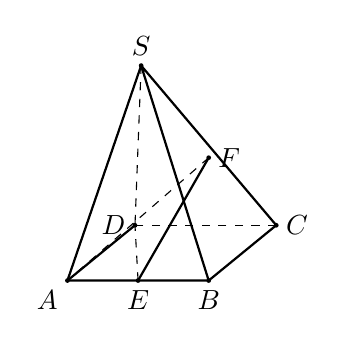
\begin{tikzpicture}[>=stealth,scale=0.78]
  \coordinate (A) at (0,0); \coordinate (B) at (2.3,0);
  \coordinate (C) at (3.4,0.9); \coordinate (D) at (1.1,0.9);
  \coordinate (S) at (1.2,3.5); \coordinate (E) at (1.15,0);
  \coordinate (F) at (2.3,2.0);
  \draw[thick] (A)--(B)--(C); \draw[dashed] (C)--(D); \draw[thick] (D)--(A);
  \draw[thick] (S)--(A) (S)--(B) (S)--(C);
  \draw[dashed] (S)--(D);
  \draw[thick] (E)--(F);
  \draw[dashed] (E)--(D) (F)--(A);
  \fill (S) circle (1.1pt) node[above] {$S$};
  \fill (A) circle (1.1pt) node[below left] {$A$};
  \fill (B) circle (1.1pt) node[below] {$B$};
  \fill (C) circle (1.1pt) node[right] {$C$};
  \fill (D) circle (1.1pt) node[left] {$D$};
  \fill (E) circle (1.1pt) node[below] {$E$};
  \fill (F) circle (1.1pt) node[right] {$F$};
\end{tikzpicture}
\end{center}
\nopagebreak[4]
（1） 求证：$EF\parallel$ 平面 $SAD$；

（2） 设 $SD=2CD$，求二面角 $A-EF-D$ 的大小。

\Needspace{4\baselineskip}
\textbf{解析}

\gksubpart{(1)}

与全国卷Ⅱ文科第 20 题相同，坐标化可证 $EF\parallel$ 平面 $SAD$。

\gksubpart{(2)}

\Needspace{5\baselineskip}
由 $SD=2CD$，取法向量计算得到二面角满足

\nopagebreak[4]
\[
\cos\theta=\frac5{\sqrt{105}}
\]
。

\gkanswer{答案（1）：见解析版}

\gkanswer{答案（2）：二面角 $A-EF-D$ 满足 $\cos\theta=\dfrac5{\sqrt{105}}$。}

\end{answer}
\begin{answer}
\gksolhead{20}{}

\textbf{题目}：

在直角坐标系 $xOy$ 中，以 $O$ 为圆心的圆与直线 $x-\sqrt3y=4$ 相切。

（1） 求圆 $O$ 的方程；

（2） 圆 $O$ 与 $x$ 轴相交于 $A,B$ 两点，圆内的动点 $P$ 使 $|PA|,|PO|,|PB|$ 成等比数列，求 $\overrightarrow{PA}\cdot\overrightarrow{PB}$ 的取值范围。

\Needspace{4\baselineskip}
\textbf{解析}

\gksubpart{(1)}

圆心到直线 $x-\sqrt3y=4$ 的距离为 $4/2=2$，故圆方程为 $x^2+y^2=4$。

\gksubpart{(2)}

\Needspace{5\baselineskip}
设圆与 $x$ 轴交点横坐标为 $\pm2$。等比条件平方化简为 $x^2-y^2=2$，而圆内条件给出 $y^2<1$。又

\nopagebreak[4]
\[
\overrightarrow{PA}\cdot\overrightarrow{PB}=x^2+y^2-4=2y^2-2
\]
，

故取值范围为 $(-2,0)$。

\gkanswer{答案（1）：圆为 $x^2+y^2=4$。}

\gkanswer{答案（2）：$\overrightarrow{PA}\cdot\overrightarrow{PB}\in\left(-\dfrac45,\dfrac45\right)$。}

\end{answer}
\begin{answer}
\gksolhead{21}{}

\textbf{题目}：

设数列 $\{a_n\}$ 的首项 $a_1\in(0,1)$，$a_n=\dfrac{3-a_{n-1}}2$，$n=2,3,4,\ldots$。

（1） 求 $\{a_n\}$ 的通项公式；

（2） 设 $b_n=a_n\sqrt{3-2a_n}$，证明 $b_n<b_{n+1}$，其中 $n$ 为正整数。

\Needspace{4\baselineskip}
\textbf{解析}

\gksubpart{(1)}

\Needspace{5\baselineskip}
令 $c_n=a_n-1$，则 $c_n=-c_{n-1}/2$，所以

\nopagebreak[4]
\[
a_n=1+(a_1-1)\left(-\frac12\right)^{n-1}
\]
。

\gksubpart{(2)}

\Needspace{5\baselineskip}
令 $\phi(t)=t^2(3-2t)$，则 $b_n^2=\phi(a_n)$。递推关系给出

\nopagebreak[4]
\[
\phi\left(\frac{3-t}{2}\right)-\phi(t)
=\frac94t(t-1)^2>0
\]
，

从而 $b_n<b_{n+1}$。

\gkanswer{答案（1）：$a_n=1+(a_1-1)\left(-\dfrac12\right)^{n-1}$。}

\gkanswer{答案（2）：$b_n<b_{n+1}$。}

\end{answer}
\begin{answer}
\gksolhead{22}{}

\textbf{题目}：

已知函数 $f(x)=x^3-x$。

（1） 求曲线 $y=f(x)$ 在点 $M(t,f(t))$ 处的切线方程；

（2） 设 $a>0$，如果过点 $(a,b)$ 可作曲线 $y=f(x)$ 的三条切线，证明：$-a<b<f(a)$。

\Needspace{4\baselineskip}
\textbf{解析}

\gksubpart{(1)}

\Needspace{5\baselineskip}
曲线 $y=x^3-x$ 在 $M(t,f(t))$ 处的切线为

\nopagebreak[4]
\[
y-(t^3-t)=(3t^2-1)(x-t)
\]
。

\gksubpart{(2)}

\Needspace{5\baselineskip}
切线过 $(a,b)$ 时参数 $t$ 满足

\nopagebreak[4]
\[
b=(3t^2-1)a-2t^3
\Longleftrightarrow 2t^3-3at^2+a+b=0
\]
。

\Needspace{5\baselineskip}
若有三条切线，则此三次式在 $0,a$ 处的极值须异号，即

\nopagebreak[4]
\[
a+b>0,\qquad b-(a^3-a)<0
\]
。

因此 $-a<b<a^3-a=f(a)$。

\gkanswer{答案（1）：切线为 $y=(3t^2-1)x-2t^3$。}

\gkanswer{答案（2）：见解析版}

\end{answer}